\documentclass[a4paper,12pt,oneside]{scrreprt}
%% Pakete:
\usepackage[utf8]{inputenc}
\usepackage[T1]{fontenc}    
\usepackage{graphicx}       
\usepackage[british,UKenglish]{babel} 
\usepackage{csquotes} 
\usepackage{eurosym}
\usepackage[linktocpage=true]{hyperref} 
\usepackage[bindingoffset=8mm]{geometry}
\usepackage{caption}
\usepackage[onehalfspacing]{setspace}
\usepackage{minted}
\usepackage[a-2b,mathxmp]{pdfx}[2018/12/22]
\usepackage[style=apa,citestyle=apa,backend=biber]{biblatex}
\addbibresource{Zotero.bib}

%% Einstellungen:
\setcounter{secnumdepth}{4}
\setcounter{tocdepth}{4}   % Tiefe der Gliederung im Inhaltsverzeichnis
\captionsetup{format=hang, justification=raggedright}
\setlength{\parindent}{0pt}

\begin{document}
\thispagestyle{empty}
\begin{titlepage}
  \begin{flushright}
  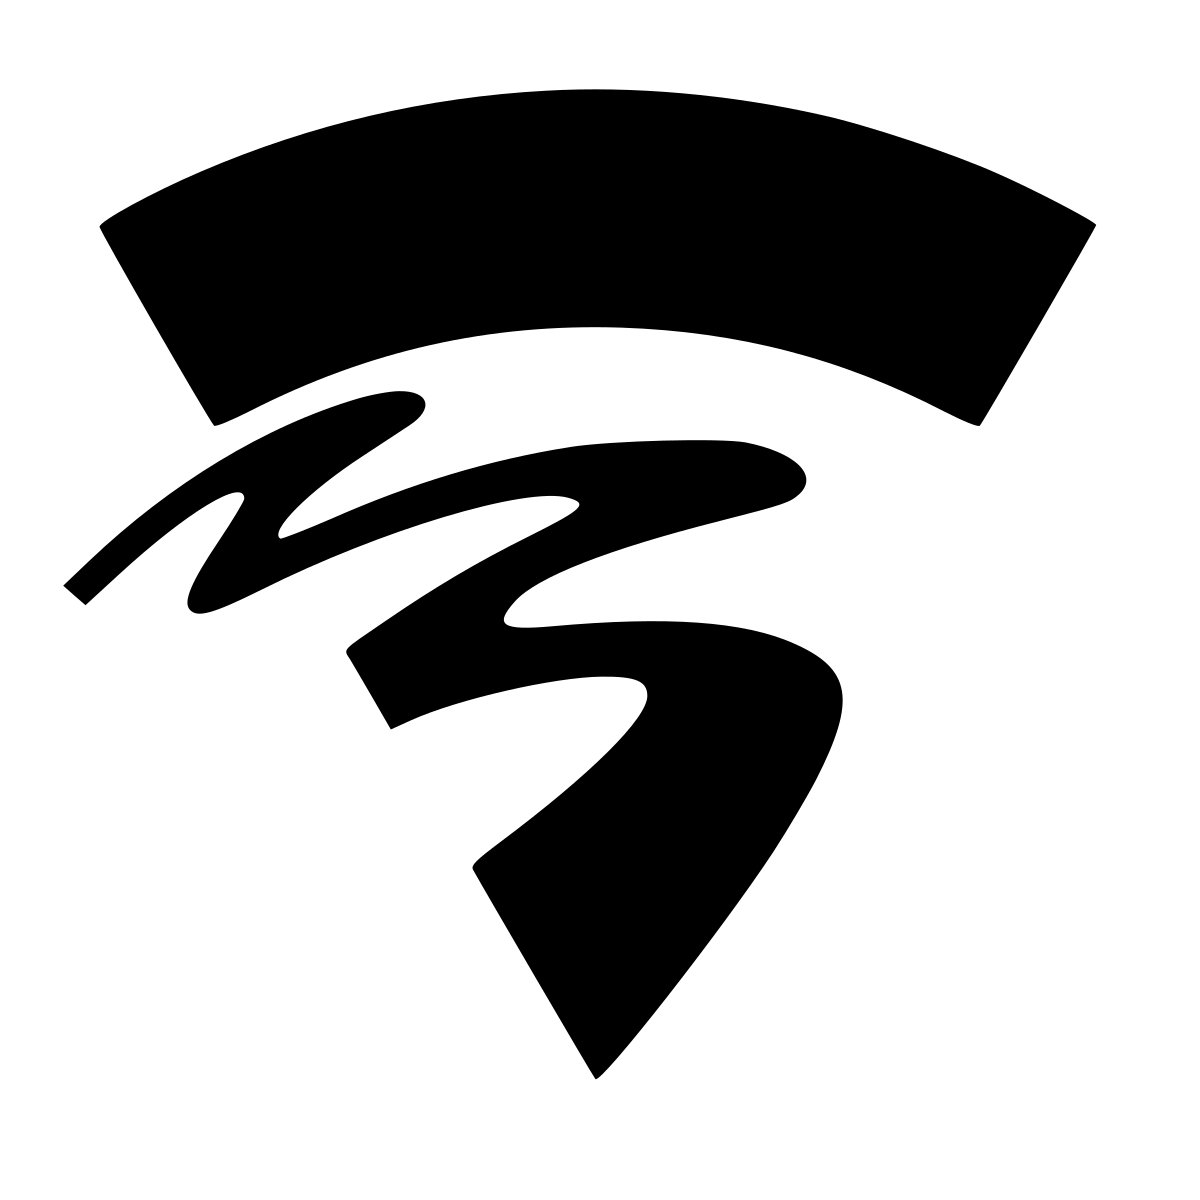
\includegraphics[width=0.3\linewidth]{images/Hogeschool_van_amsterdam_logo.svg}
  \end{flushright}
  \begin{flushleft}
  \section*{R\&D Assignment}
  \subsection*{3D Dungeon Generator}

  \vspace{1cm}
  Hogeschool van Amsterdam\newline
  Gameplay Engineering

  \vspace{0.5cm}

  Michael Spiegel\newline
  04.10.2022
  \end{flushleft}
\end{titlepage}

% Table of Contents:
\tableofcontents

% Content:
\chapter{Introduction}
For my research project I chose a 3D dungeon generator that should generate a new dungeon every time the game is started. Furthermore, I decided to make it possible to walk through the dungeon. For this I want to add a player that will be placed in a randomly chosen start room. To make the whole dungeon more interesting and not leave it as an empty place, I plan to add some scenery like torches. Additionally the dungeon should also contain enemies for which I try to implement a combat system. The focus lies on a performant generation of the dungeon and on the look. Through this project I want to understand how the algorithms work that are used for dungeon generation. Furthermore, I want to get knowledge about combat systems in games.

\chapter{Existing algorithms for dungeon generation}
There exist several algorithms which can be used to create dungeons. In this chapter three algorithms will be described and in the end compared. 

\section{Binary Space Partitioning}
The binary space partitioning algorithm is very popular for creating dungeons because it is a fast algorithm and not that hard to implement. With this algorithm the dungeon is represented through a binary tree structure. The initial space will be split in each iteration of the algorithm. With this algorithm it is possible to create a variety of dungeons each time the code is run. For this it is necessary that specific parts of the split have to be randomised. The split can be horizontal or vertical. Figure \ref{fig:bsp_example} shows how a dungeon generated with Binary Space Partitioning looks like. (\cite[][]{williams_investigation_nodate})

\begin{figure}[htb]
\centering
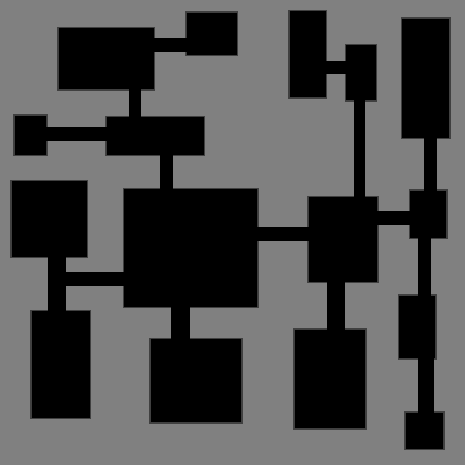
\includegraphics[scale=0.5]{images/bsp_example.png} 
\caption{Example of a BSP generated dungeon}
Source: \cite[][]{williams_investigation_nodate}
\label{fig:bsp_example}
\end{figure}

\newpage
\section{Cellular Automata}
The Cellular automata algorithm uses a grid of cells to build a dungeon. Each cell has a reference to its neighbour cells and a defined state for the time $t = 0$. With the help of predefined rules the state for $t = t + 1$ can be calculated. Depending on the defined rules and the cell states there will be patterns that occur from time to time. A cell it self represents a space where the player can walk but also a space where the player can not walk for example rocks. As you can see in figure \ref{fig:cellular_automata_example} Cellular Automata creates more cave like dungeons without real rooms. (\cite[][]{williams_investigation_nodate})

\begin{figure}[htb]
\centering
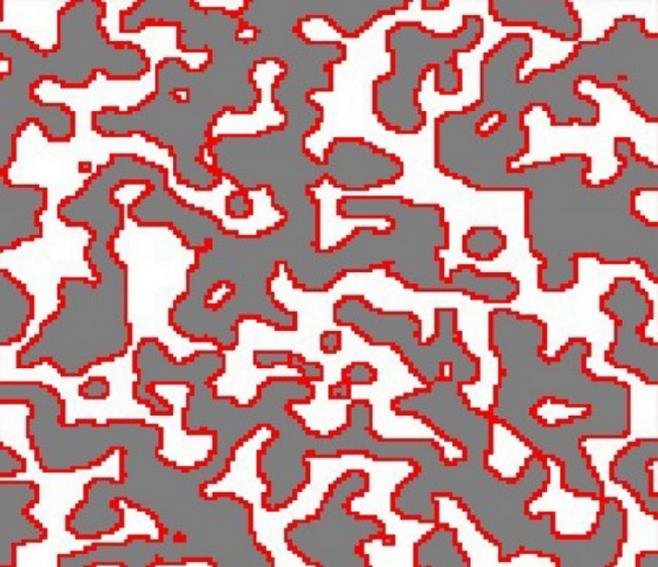
\includegraphics[scale=0.5]{images/cellular_automata_example.png} 
\caption{Example of a Cellular Automata generated dungeon}
Source: \cite[][]{williams_investigation_nodate}
\label{fig:cellular_automata_example}
\end{figure}

\newpage
\section{Delaunay Triangulation}
The last algorithm is the delaunay triangulation algorithm for dungeon generation. This algorithm also uses cells but in this case a random rectangle is created inside of each cell. After this step the algorithm separates the room and prevents them from overlapping. All cells that are exceeding a threshold become rooms. To connect all rooms a graph for all the room centre points is constructed. Additionally to the delaunay triangulation algorithm it is necessary to generate a minimum spanning tree of the originally create graph to remove cycles. In figure \ref{fig:delaunay_example} you can see how a dungeon generated with the delaunay triangulation looks like. Compared to the other two algorithms it is more similar to the result of the binary space partition generated dungeon because both use rooms. (\cite[][]{williams_investigation_nodate})

\begin{figure}[htb]
\centering
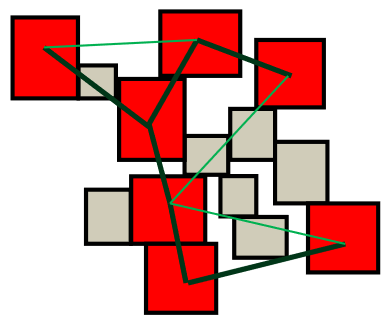
\includegraphics[scale=0.5]{images/delaunay_example.png} 
\caption{Example of a Delaunay Triangulation generated dungeon}
Source: \cite[][]{williams_investigation_nodate}
\label{fig:delaunay_example}
\end{figure}

\section{Comparison of the algorithms}
Now let's compare those algorithms to explain which one fits best for the purpose of this project. The cellular automata algorithm generates more cave like dungeons which is not applicable to the goal of this project. The dungeon should consist of rooms which only the binary space partition and the delaunay triangulation algorithm provides. 
\\
\\
To compare those two algorithms let's have a look on the performance. Figure \ref{fig:bsp_performance} shows the performance of the binary space partitioning algorithm. This algorithm is slow when less rooms are used for the dungeon but has its strength in the generation of more complex dungeons that consists of a huge amount of rooms.  
\begin{figure}[htb]
\centering
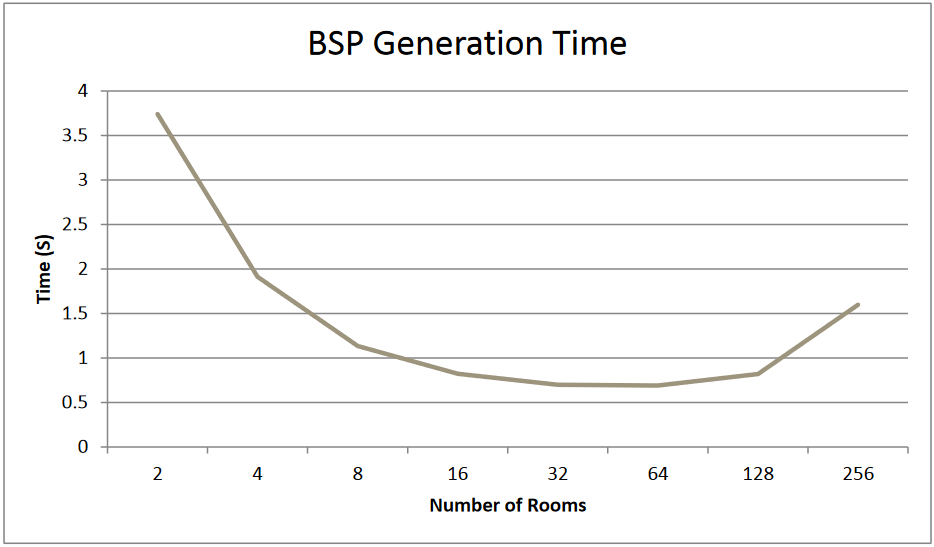
\includegraphics[scale=0.5]{images/bsp_performance.png} 
\caption{Performance of the Binary Space Partitioning algorithm}
Source: \cite[][]{williams_investigation_nodate}
\label{fig:bsp_performance}
\end{figure}

Figure \ref{fig:delaunay_performance} show that compared to the other algorithm the delaunay triangulation algorithm is faster when it comes to dungeons with less rooms. On the other side this algorithm gets slower with the increasing amount of rooms. This means, that this algorithm fits best if the dungeon will only consist of a few rooms.
\begin{figure}[htb]
\centering
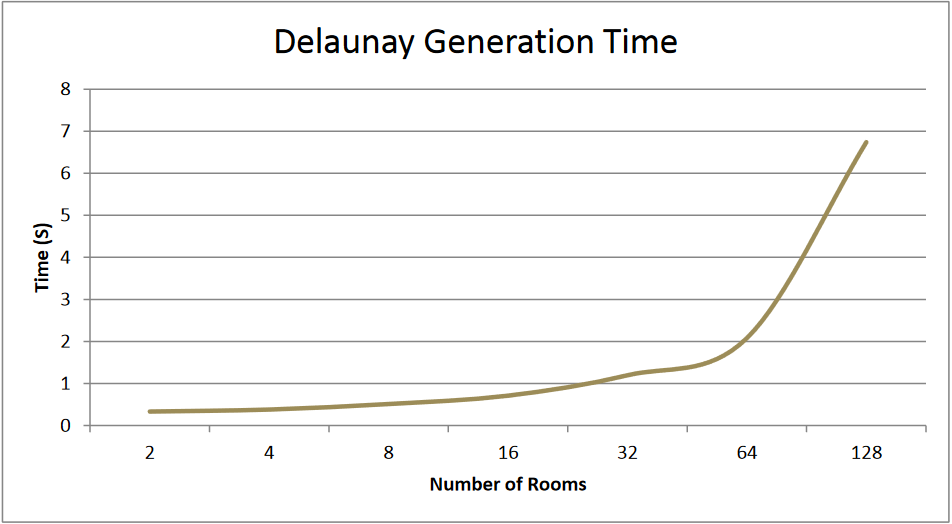
\includegraphics[scale=0.5]{images/delaunay_performance.png} 
\caption{Performance of the Delaunay Triangulation algorithm}
Source: \cite[][]{williams_investigation_nodate}
\label{fig:delaunay_performance}
\end{figure}

% List of Figures:
\clearpage
\phantomsection
\addcontentsline{toc}{chapter}{List of Figures}
\listoffigures

% Bibliography:
\clearpage
\phantomsection
\addcontentsline{toc}{chapter}{Bibliography}
\printbibliography

\end{document}
